\chapter{Simulado 1}

\chapter{Simulado 1}

\num{1} Gabriel durante sua aula estava aprendendo a montar números
utilizando o material dourado e montou a seguinte número?

\begin{figure}[htpb!]
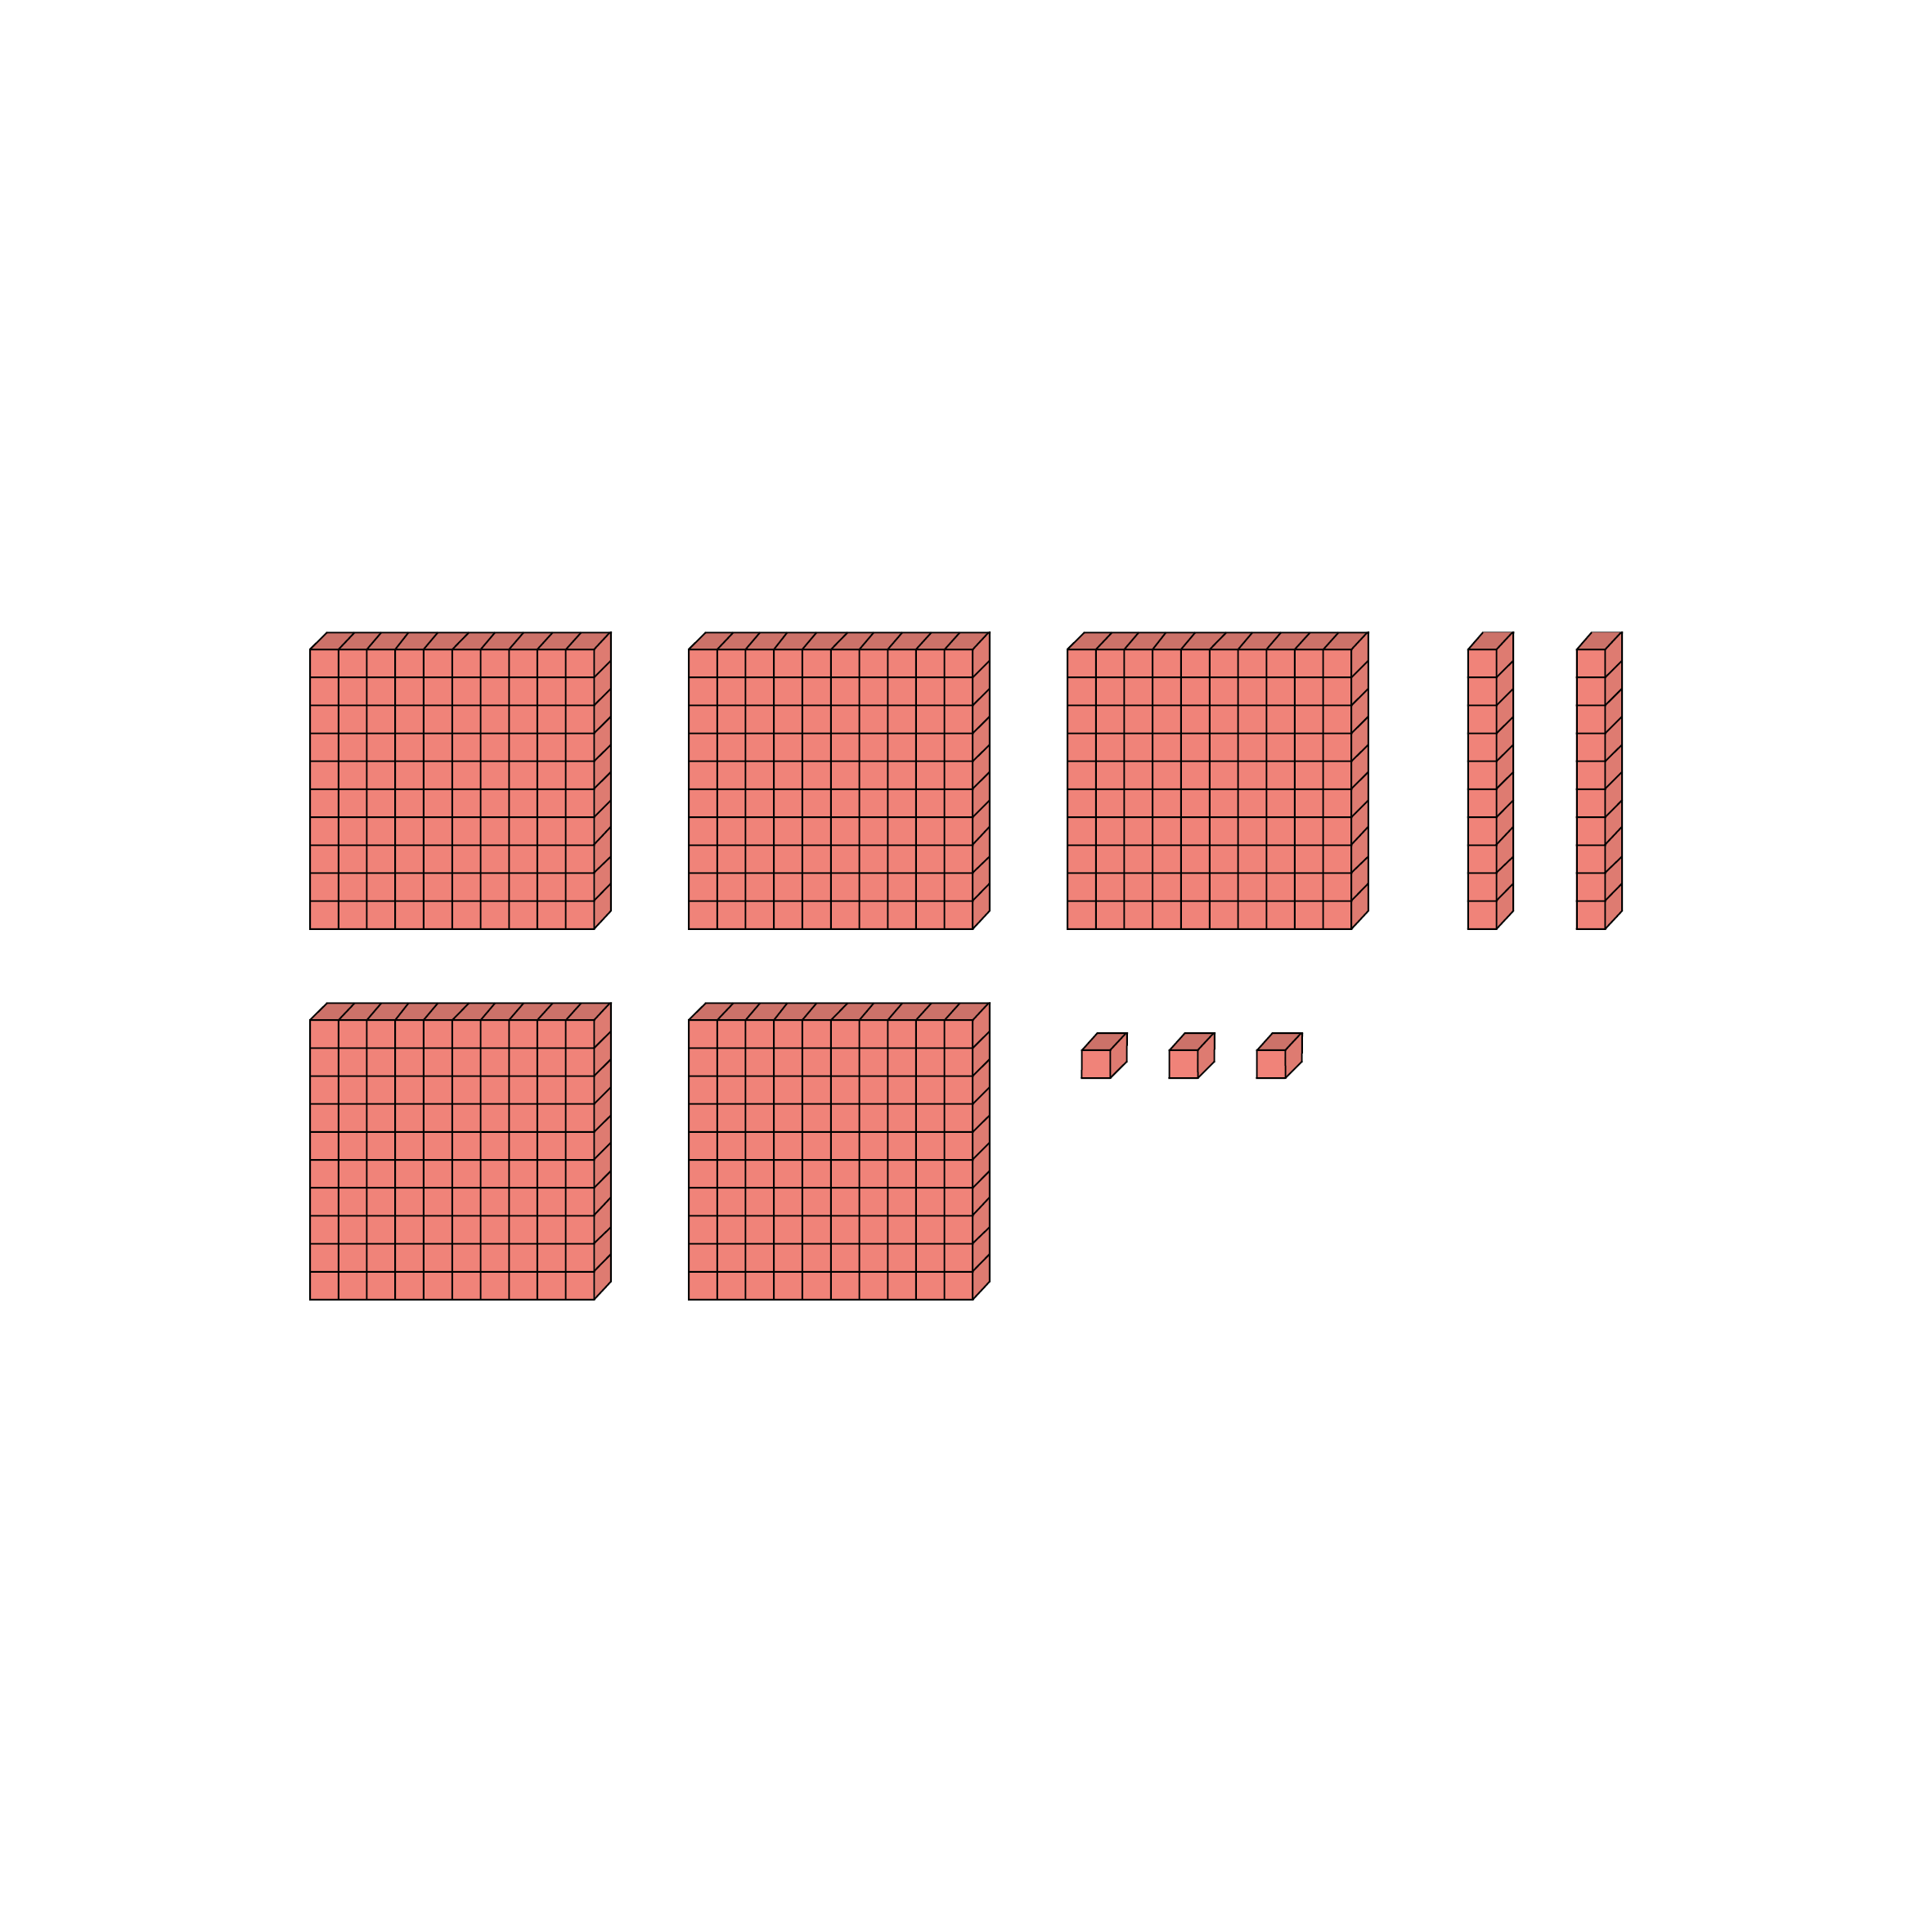
\includegraphics[width=\textwidth]{../ilustracoes/MAT5/SAEB_5ANO_MAT_figura112.png}
\end{figure}

Qual é o número representado pelo material dourado na figura acima?

\begin{escolha}
\item
  623
\item
  423
\item
  503
\item
  523
\end{escolha}

\coment{SAEB: Compor ou decompor números naturais de até 6
ordens na forma aditiva, ou em suas ordens, ou em adições e 
multiplicações.

BNCC: EF05MA01 - Ler, escrever e ordenar números naturais até a ordem das 
centenas de milhar com compreensão das principais características do 
sistema de numeração decimal. 
EF05MA10 - Concluir, por meio de investigações, que a relação de 
igualdade existente entre dois membros permanece ao adicionar, subtrair, 
multiplicar ou dividir cada um desses membros por um mesmo número, para 
construir a noção de equivalência.
EF05MA11 - Resolver e elaborar problemas cuja conversão em sentença 
matemática seja uma igualdade com uma operação em que um dos termos é 
desconhecido.

Para encontrar a resposta, é preciso verificar que cada um dos 
cinco grandes cubos é composto por cem unidades. À direita, cada uma das 
duas colunas tem dez unidades. Finalmente, cada cubinho pequeno 
corresponde a apenas uma unidade. Dessa maneira, somam-se as cem unidades 
dos grandes cubos, com as vinte das colunas e as três dos cubinhos: 5 x 
100 + 2 x 10 + 3 x 1 = 523.  
a) Incorreta. O número correto é 523, não 623.
b) Incorreta. O número correto é 523, não 423.
c) Incorreta. O número correto é 523, não 503.
d) Correta. 5 x 100 + 2 x 10 + 3 x 1 = 523.}

\num{2} Alex estava jogando dardos em um alvo que possuía áreas de
pontuação e durante uma rodada notou que a expressão 2 x 1.000 + 3 x 100
+ 1 x 10, quando resolvida, gerava exatamente o número de pontos que ele
havia feito naquela rodada. A pontuação de Alex naquela rodado foi:

\begin{escolha}
\item
  231 pontos
\item
  2.031 pontos
\item
  2.301 pontos
\item
  2.310 pontos
\end{escolha}

\coment{SAEB: Compor ou decompor números naturais de até 6 ordens na
forma aditiva, ou em suas ordens, ou em adições e multiplicações.

BNCC: EF05MA01 - Ler, escrever e ordenar números naturais até a ordem das 
centenas de milhar com compreensão das principais características do 
sistema de numeração decimal. 
EF05MA10 - Concluir, por meio de investigações, que a relação de 
igualdade existente entre dois membros permanece ao adicionar, subtrair, 
multiplicar ou dividir cada um desses membros por um mesmo número, para 
construir a noção de equivalência.
EF05MA11 - Resolver e elaborar problemas cuja conversão em sentença 
matemática seja uma igualdade com uma operação em que um dos termos é 
desconhecido.

Para obter a resposta correta, basta solucionar a expressão numérica.
a) Incorreta. (2 x 1.000) + (3 x 100) + (1 x 10) = 2.310.
b) Incorreta. (2 x 1.000) + (3 x 100) + (1 x 10) = 2.310.
c) Incorreta. (2 x 1.000) + (3 x 100) + (1 x 10) = 2.310.
d) Correta. (2 x 1.000) + (3 x 100) + (1 x 10) = 2.310.}

\num{3} A escola em que Jack estuda está promovendo uma conscientização de
preservação do meio ambiente através do plantio de mudas de árvores
nativas. Sabe-se que já foram plantadas 359 mudas e ainda serão
plantadas 246. Quantas mudas ao todo serão plantadas durante esse evento
da escola de Jack?

\begin{escolha}
\item
  513
\item
  523
\item
  605
\item
  705
\end{escolha}

\coment{SAEB: Determinar o número desconhecido que torna verdadeira
uma igualdade que envolve as operações fundamentais com números naturais
de até 6 ordens.

BNCC: EF05MA01 - Ler, escrever e ordenar números naturais até a ordem das 
centenas de milhar com compreensão das principais características do 
sistema de numeração decimal. 
EF05MA10 - Concluir, por meio de investigações, que a relação de 
igualdade existente entre dois membros permanece ao adicionar, subtrair, 
multiplicar ou dividir cada um desses membros por um mesmo número, para 
construir a noção de equivalência.
EF05MA11 - Resolver e elaborar problemas cuja conversão em sentença 
matemática seja uma igualdade com uma operação em que um dos termos é 
desconhecido.

a) Incorreta. 359 + 246 = 605, não 513.
b) Incorreta. 359 + 246 = 605, não 523.
c) Correta. 359 + 246 = 605.
d) Incorreta. 359 + 246 = 605, não 705.}

\num{4} Na escola em que André estuda há 4.054 alunos. Já na escola 
em que Pedro estuda estão matriculados 2.843 alunos. Se, no próximo ano,
300 alunos se matricularem em cada uma das escolas, qual será a diferença
entre a quantidade de alunos das duas escolas?

\begin{escolha}
\item
  2.416
\item
  1.211
\item
  1.883
\item
  1.463
\end{escolha}

\coment{SAEB: Determinar o número desconhecido que torna verdadeira
uma igualdade que envolve as operações fundamentais com números naturais
de até 6 ordens.

BNCC: EF05MA01 - Ler, escrever e ordenar números naturais até a ordem das 
centenas de milhar com compreensão das principais características do 
sistema de numeração decimal. 
EF05MA10 - Concluir, por meio de investigações, que a relação de 
igualdade existente entre dois membros permanece ao adicionar, subtrair, 
multiplicar ou dividir cada um desses membros por um mesmo número, para 
construir a noção de equivalência.
EF05MA11 - Resolver e elaborar problemas cuja conversão em sentença 
matemática seja uma igualdade com uma operação em que um dos termos é 
desconhecido.

a) Incorreta. 4.054 -- 2.843 = 1.211, não 2.416.
b) Correta. 4.054 -- 2.843 = 1.211. Como o aumento foi o mesmo
nos dois números, não precisamos somar 300 aos números
antigos já que a diferença entre eles se manterá a mesma.
c) Incorreta. 4.054 -- 2.843 = 1.211, não 1.883.
d) Incorreta. 4.054 -- 2.843 = 1.211, não 1.463.}

\num{5} A numeração das salas de um novo prédio comercial de 5 andares
segue a numeração dos andares e a orientação da árvore que se
localiza ao lado do prédio. Assim, em cada andar a numeração começa pela
sala mais próxima da árvore da seguinte maneira: 101, 102, 103; 201, 202, 
203 --- e assim sucessivamente, até o quinto andar.

\begin{figure}[htpb!]
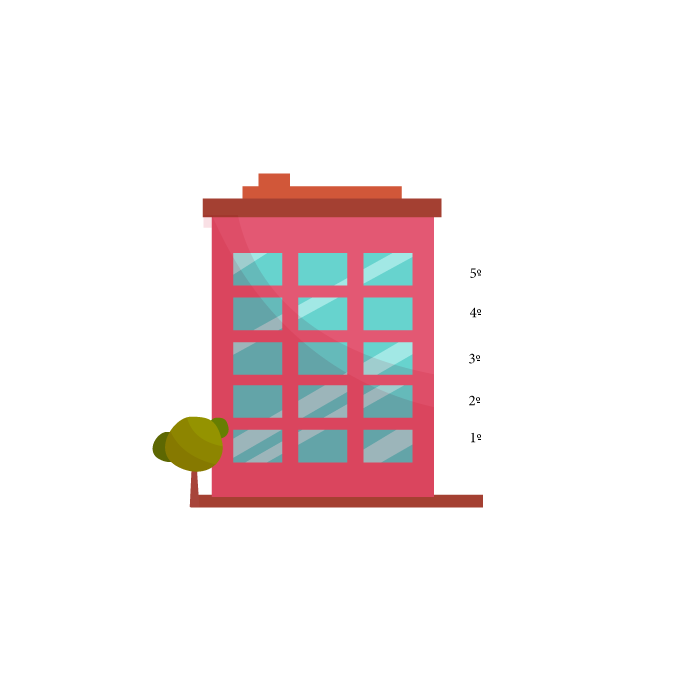
\includegraphics[width=\textwidth]{../ilustracoes/MAT5/SAEB_5ANO_MAT_figura113.png}
\end{figure}

Qual a numeração da sala do 3º andar que está com a janela fechada?

\begin{escolha}
\item
  301
\item
  302
\item
  303
\item
  304
\end{escolha}

\coment{SAEB: Inferir o padrão ou a regularidade de uma sequência de
números naturais ordenados, objetos ou figuras. 

a) Incorreta. 301 é o número da sala mais próxima da árvore.
b) Incorreta. 302 é o número da sala intermediária do terceiro andar.
c) Correta. De acordo com as orientações do enunciado, a sala mais
próxima da árvore será indicada com o final 1. A mais distante, com o 
final 3. Dessa maneira, o número da sala de janela fechada do terceiro 
andar --- iniciado com o número 3, seguido de zero --- é 303.
d) Incorreta. Existem apenas 3 salas por andar, de modo que não pode
haver sala de número 304.}

\num{6} Ernesto comprou, para a festa de aniversário de sua filha, 
8 litros de refrigerante e copos descartáveis com capacidade de 200
mililitros cada. Quantos copos, com a capacidade máxima tomada por
refrigerante, poderão ser servidos nessa festa considerando que Ernesto 
não comprará mais refrigerante?

\begin{escolha}
\item
  16
\item
  20
\item
  32
\item
  40
\end{escolha}

\coment{SAEB: Resolver problemas de multiplicação ou de divisão,
envolvendo números naturais de até 6 ordens, com os significados de
formação de grupos iguais (incluindo repartição equitativa e medida),
proporcionalidade ou disposição retangular.

a) Incorreta. O número máximo de copos que poderão ser servidos é 40, não
16.
b) Incorreta. O número máximo de copos que poderão ser servidos é 40, não 20.
c) Incorreta. O número máximo de copos que poderão ser servidos é 40, não 32.
d) Correta. 8 litros correspondem a 8.000 ml de refrigerante que foram
comprados. É possível obter o número máximo de copos que poderão ser
servidos dividindo a quantidade de litros pela capacidade máxima de 
cada copo: 8.000/200 = 40.}

\num{7} Observe a figura abaixo:

\begin{figure}[htpb!]
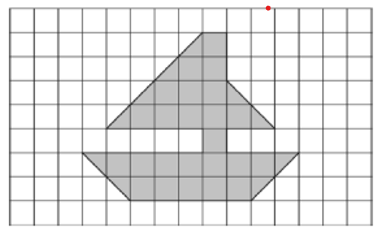
\includegraphics[width=.5\textwidth]{./imgs/mat19.png}
\end{figure}

Considerando tudo que está pintado, juntando duas metades de quadradinhos 
para formar um completo, quantos quadradinhos estão pintados?

\begin{escolha}
\item
  24
\item
  26
\item
  29
\item
  34
\end{escolha}

\coment{SAEB: Medir ou comparar perímetro ou área de figuras planas
desenhadas em malha quadriculada.

a) Incorreta. O número total de quadradinhos é 29, não 24.
b) Incorreta. O número total de quadradinhos é 29, não 26.
c) Incorreta. Primeiramente, é preciso contar os quadradinhos completos, 
que são 24. Depois, contar os quadradinhos que estão pela metade (10) e 
dividir esse número por 2: 10/2 = 5. Vinte e quatro quadradinhos 
completos + 10 metades (que correspondem a 5 completos) = 29 quadradinhos 
no total. 
d) Incorreta. O número total de quadradinhos é 29, não 34.}

\num{8} Ana Beatriz e Camila juntaram todo dinheiro que ganharam de seus
pais no último mês. As quantias estão representadas na figura abaixo:

\begin{figure}[htpb!]
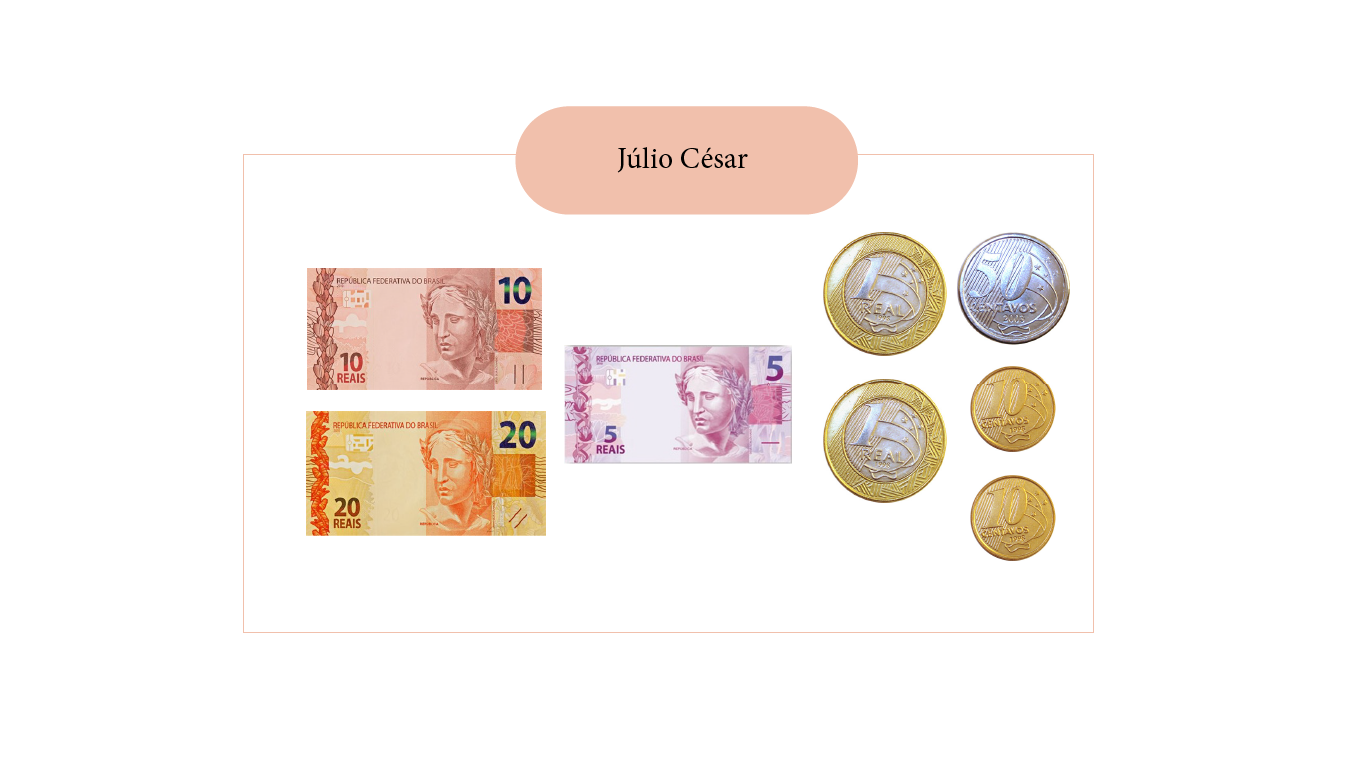
\includegraphics[width=.5\textwidth]{../ilustracoes/MAT5/SAEB_5ANO_MAT_figura114a.png}
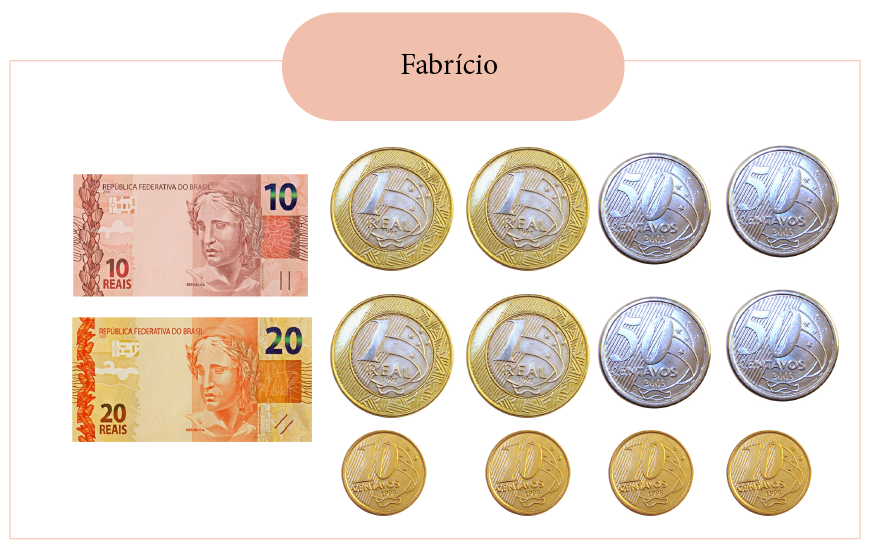
\includegraphics[width=.5\textwidth]{../ilustracoes/MAT5/SAEB_5ANO_MAT_figura114b.png}
\end{figure}
%Colocar Ana Beatriz no lugar de Júlio Cesar e Camila no lugar de Fabrício

Somando-se os dois valores, qual o valor total que as duas conseguiram
juntar?

\begin{escolha}
\item
  R\$ 36,40
\item
  R\$ 37,70
\item
  R\$ 74,10
\item
  R\$ 85,20
\end{escolha}

\coment{SAEB: Relacionar valores de moedas e/ou cédulas do sistema
monetário brasileiro, com base nas imagens desses objetos.

a) Incorreta. O valor total é de R\$ 74,10.
b) Incorreta. O valor total é de R\$ 74,10.  
c) Correta. Ana Beatriz tem, em cédulas, R\$ 20,00 + 10,00 + 5,00; em
moedas R\$ 2,70, em um total de R\$ 37,70. Camila tem R\$ 20,00 + 10,00 
em cédulas e R\$ 6,40 em moedas: R\$ 36,40. Juntas, elas têm R\$ 37,70 + 
36,40 = R\$ 74,10.   
b) Incorreta. O valor total é de R\$ 74,10.}

\num{9} A mãe de Isabeli está esperando um bebê e hoje será o dia de
descobrir se será menina ou menino. Qual a probabilidade de Isabeli ter
uma irmã?

\begin{escolha}
\item
  0\%
\item
  25\%
\item
  50\%
\item
  100\%
\end{escolha}

\coment{SAEB: Determinar a probabilidade de ocorrência de um
resultado em eventos aleatórios, quando todos os resultados possíveis
têm a mesma chance de ocorrer (equiprováveis).

BNCC: EF05MA22 - Apresentar todos os possíveis resultados de um experimento aleatório, estimando se esses resultados são igualmente prováveis ou não. 
EF05MA23 - Determinar a probabilidade de ocorrência de um resultado em eventos aleatórios, quando todos os resultados possíveis têm a mesma chance de ocorrer (equiprováveis).

a) Incorreta. A probabilidade é de 50\%.
b) Incorreta. A probabilidade é de 50\%. 
c) Correta. Como nesse evento só existem duas possibilidades (menino ou
menina), a probabilidade de Isabeli ter uma irmã é de 50\%.
d) Incorreta. A probabilidade é de 50\%.}

\num{10} O gráfico abaixo mostra a taxa de desemprego de uma grande cidade
brasileira:

%Não gosto desse gráfico: iniciado em março, ele induz ao erro. O próprio autor da questão caiu nessa armadilha. Tive de refazer o gabarito. 

\begin{figure}[htpb!]
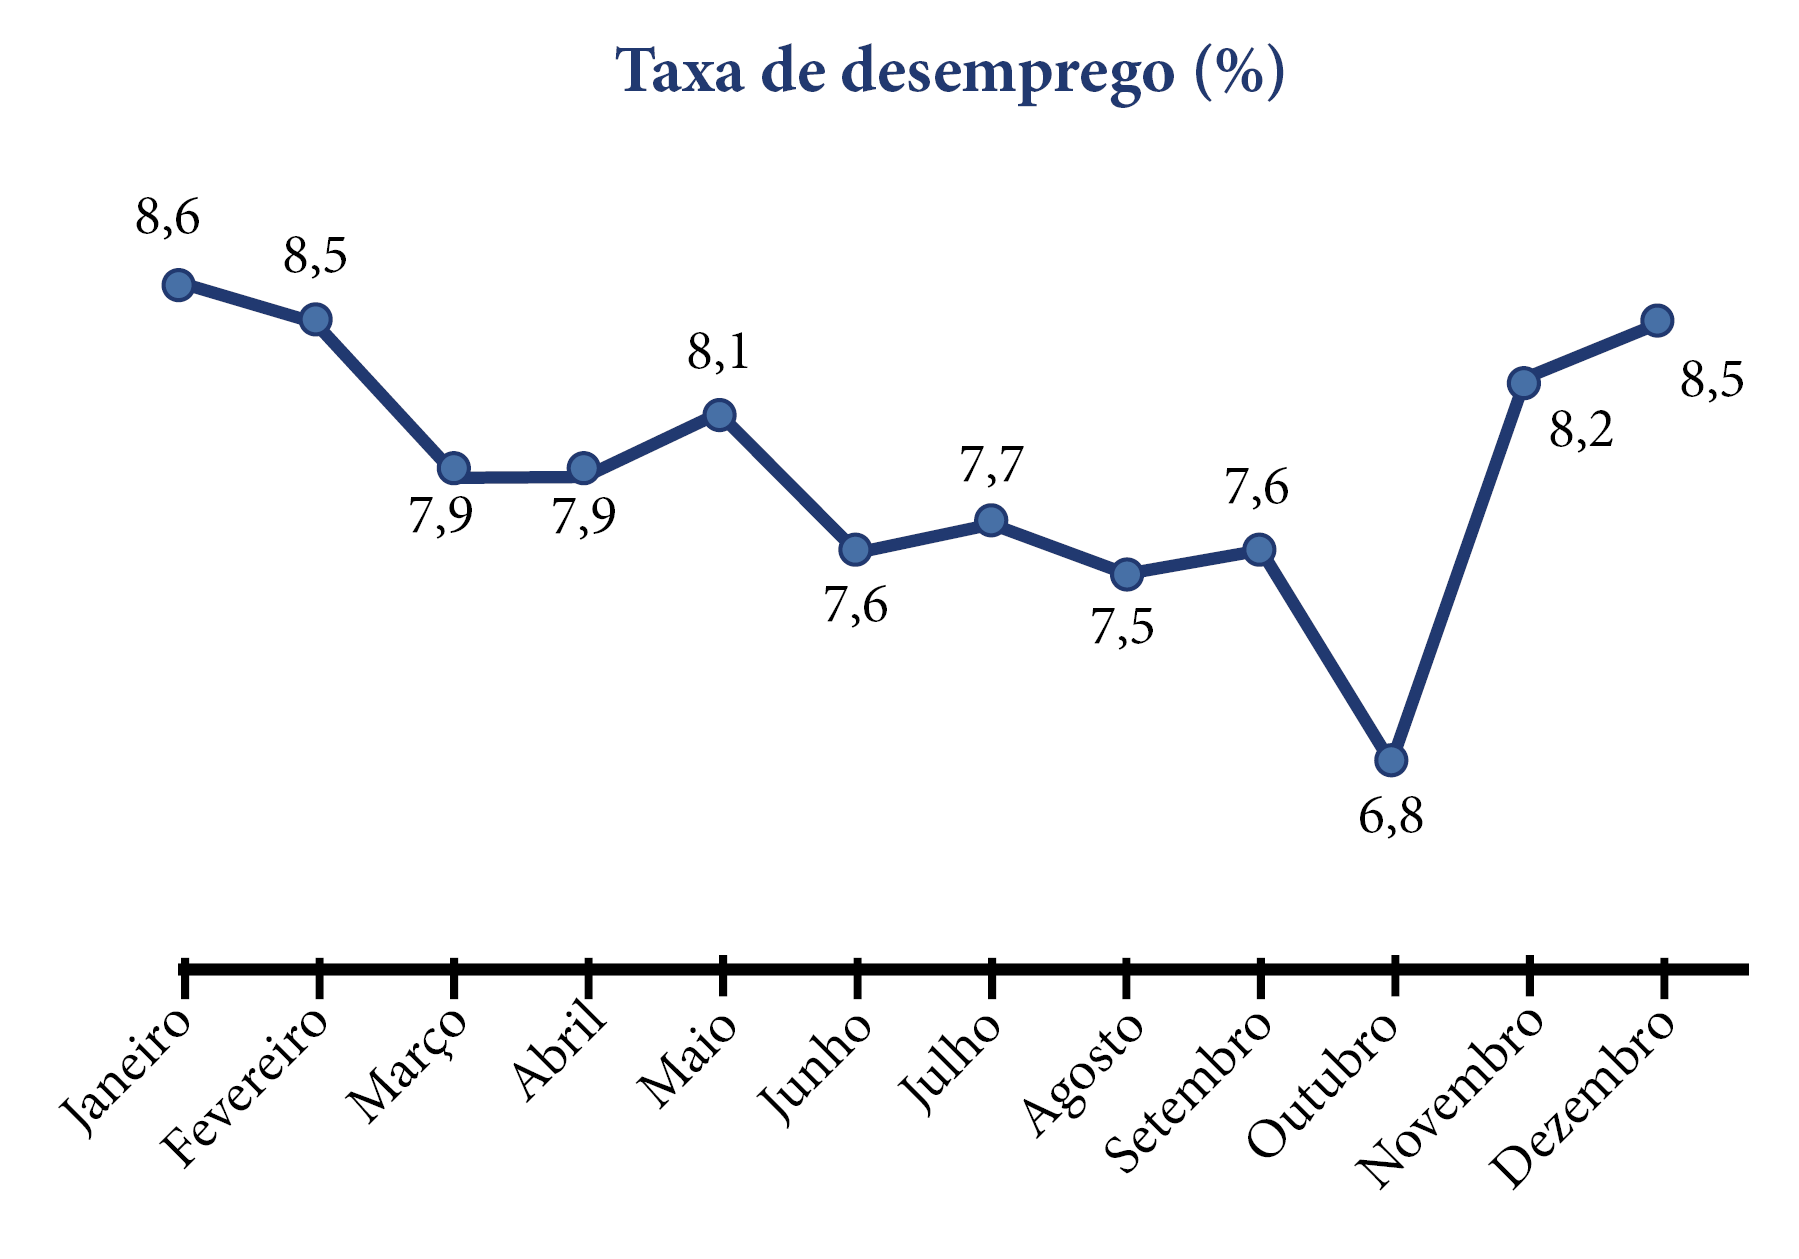
\includegraphics[width=\textwidth]{../ilustracoes/MAT5/SAEB_5ANO_MAT_figura115.png}
\end{figure}

Por meio da análise do gráfico, o mês que apresentou menor índice de
desemprego foi:

\begin{escolha}
\item
  Março
\item
  Julho
\item
  Outubro
\item
  Dezembro
\end{escolha}

\coment{SAEB: Resolver problemas que envolvam dados apresentados
tabelas (simples ou de dupla entrada) ou gráficos estatísticos (barras
simples ou agrupadas, colunas simples ou agrupadas, pictóricos ou de
linhas).

BNCC: EF05MA24 - Interpretar dados estatísticos apresentados em textos, tabelas e gráficos (colunas ou linhas), referentes a outras áreas do conhecimento ou a outros contextos, como saúde e trânsito, e produzir textos com o objetivo de sintetizar conclusões.

a) Incorreta. Em março o índice foi de 8,6\%, maior do que os 6,8\% de dezembro. 
b) Incorreta. Em julho o índice foi de 8,1\%, maior do que os 6,8\% de dezembro.
c) Incorreta. Em outubro o índice foi de 7,5\%, maior do que os 6,8\% de dezembro.
d) Correta. Analisando o gráfico, verifica-se que a menor taxa de 
desemprego ocorreu em dezembro, com 6,8\%.}

\num{11} Em uma rua de comprimento AB, seis árvores serão plantadas de 
forma equidistante, em reta numérica, conforme a figura:

\begin{figure}[htpb!]
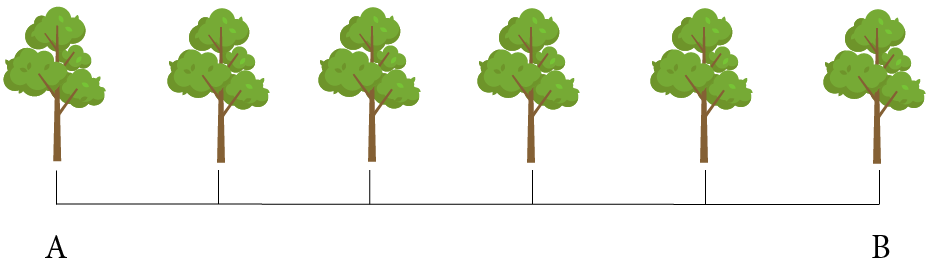
\includegraphics[width=\textwidth]{../ilustracoes/MAT5/SAEB_5ANO_MAT_figura116.png}
\end{figure}

Qual a fração representada pela distância entre a segunda e a terceira 
árvores em relação ao tamanho total?

\begin{escolha}
\item
  1/4
\item
  2/3
\item
  1/3
\item
  1/5
\end{escolha}

\coment{SAEB: Representar frações menores ou maiores que a unidade
(por meio de representações pictóricas) ou associar frações a
representações pictóricas.

BNCC: EF05MA03 - Identificar e representar frações (menores e maiores que a unidade), associando-as ao resultado de uma divisão ou à ideia de parte de um todo, utilizando a reta numérica como recurso.

EF05MA04 - Identificar frações equivalentes.

EF05MA06 - Associar as representações 10\%, 25\%, 50\%, 75\% e 100\% respectivamente à décima parte, quarta parte, metade, três quartos e um inteiro, para calcular porcentagens, utilizando estratégias pessoais, cálculo mental e calculadora, em contextos de educação financeira, entre outros.

a) Incorreta. Como a distância total entre as seis árvores está dividida 
em 5 partes iguais, a fração será 1/5 (não 1/4).
b) Incorreta.  Como a distância total entre as seis árvores está dividida 
em 5 partes iguais, a fração será 1/5 (não 2/3)
c) Incorreta.  Como a distância total entre as seis árvores está dividida 
em 5 partes iguais, a fração será 1/5 (não 1/3)
d) Correta. Como a distância total entre as seis árvores está dividida em 
5 partes iguais, a fração será 1/5.

BNCC: EF05MA03, EF05MA04, EF05MA06}

\num{12} Juca, a uma velocidade de 80 km/h costuma gastar 1 hora e 30
minutos para ir da cidade em que mora até a cidade em que sua avó mora.
Se ele, em certo dia, reduziu a velocidade para 60 km/h, o tempo que
gastou para ir da casa em que mora até a casa em que sua avó reside foi
de:

\begin{escolha}
\item
  1 horas
\item
  1 horas e 7 minutos
\item
  2 horas
\item
  2 horas e 15 minutos
\end{escolha}

\coment{SAEB: Resolver problemas que envolvam variação de
proporcionalidade direta entre duas grandezas.

BNCC: EF05MA12 - Resolver problemas que envolvam variação de 
proporcionalidade direta entre duas grandezas, para associar a quantidade 
de um produto ao valor a pagar, alterar as quantidades de ingredientes de 
receitas, ampliar ou reduzir escala em mapas, entre outros.

a) Incorreta. Com a redução de velocidade, o percurso terá a duração de 2 horas.
b) Incorreta. Com a redução de velocidade, o percurso terá a duração de 2 horas.
c) Correta. Como, na situação inicial, Juca percorre 80 km em uma hora,
conclui-se que em uma hora e meia ele percorre 120 km. Dessa maneira,
reduzindo a velocidade para 60 km/h, ele percorrerá 60 km em uma hora; 
mantendo-se a proporção, os 120 km serão percorridos em 2 horas.
d) Incorreta. Com a redução de velocidade, o percurso terá a duração de 2 horas.}

\num{13}De quantas maneiras diferentes, uma pessoa pode se vestir tendo à
disposição 10 camisetas e 5 bermudas?

\begin{escolha}
\item
  5
\item
  10
\item
  15
\item
  50
\end{escolha}

\coment{SAEB: Resolver problemas simples de contagem (combinatória).

BNCC: EF05MA09 - Resolver e elaborar problemas simples de contagem 
envolvendo o princípio multiplicativo, como a determinação do número de 
agrupamentos possíveis ao se combinar cada elemento de uma coleção com 
todos os elementos de outra coleção, por meio de diagramas de árvore ou 
por tabelas.

a) Incorreta. Existema 50 formas diferentes de se vestir, não 5.
b) Incorreta. Existema 50 formas diferentes de se vestir, não 10.
c) Incorreta. Existema 50 formas diferentes de se vestir, não 15.
d) Correta. Para obter o número de maneiras diferentes de se vestir, 
basta multiplicar o número de camisetas pelo de bermudas: 10 x 5 = 50.}

\num{14} 141,1 litros de suco de laranja dever ser  
colocados, igualmente, em 17 tambores. Quantos litros de suco de
laranja serão colocados em cada tambor?

\begin{escolha}
\item
  5,3 litros
\item
  6,3 litros
\item
  7,3 litros
\item
  8,3 litros
\end{escolha}

\coment{SAEB: Resolver problemas de multiplicação ou de divisão,
envolvendo números racionais apenas na representação decimal finita até
a ordem dos milésimos, com os significados de formação de grupos iguais
(incluindo repartição equitativa de medida), proporcionalidade ou
disposição retangular.

BNCC: EF05MA07 - Resolver e elaborar problemas de adição e subtração com números naturais e com números racionais, cuja representação decimal seja finita, utilizando estratégias diversas, como cálculo por estimativa, cálculo mental e algoritmos.
EF05MA08 - Resolver e elaborar problemas de multiplicação e divisão com números naturais e com números racionais cuja representação decimal é finita (com multiplicador natural e divisor natural e diferente de zero), utilizando estratégias diversas, como cálculo por estimativa, cálculo mental e algoritmos.

a) Incorreta. Cada tambor conterá 8,3 litros, não 5,3.
b) Incorreta. Cada tambor conterá 8,3 litros, não 6,3.
c) Incorreta. Cada tambor conterá 8,3 litros, não 7,3.
d) Correta. Para calcular a quantidade de litros de suco de laranja
que será colocada em cada tambor, basta dividir o número de litros pelo
de tambores: 141,1/17 = 8,3 litros.}

\num{15} Observe a imagem.
  \begin{figure}[htpb!]

\includegraphics[width=\textwidth]{./imgs/img14.jpg}
\end{figure}
%Disponível em: https://br.freepik.com/fotos-gratis/lutadores-de-karate-no-campeonato-de-luta-de-tatami\_30182444.htm\#query=jud\%C3\%B4\&position=42\&from\_view=search\&track=sph. Acesso em: 14 fev. 2023.

\noindent{}Observando os dois competidores, podemos perceber que eles estão
demostrando respeito um ao outro. O motivo é que eles estão

\begin{escolha}
\item realizando uma saudação antes de lutar.

\item usando um kimono branco.

\item praticando a luta em uma competição.

\item evitando usar golpes específicos das lutas.
\end{escolha}

\coment{SAEB: Identificar elementos constitutivos dos esportes, da ginástica e
das lutas.

BNCC: EF35EF06 -- Diferenciar os conceitos de jogo e esporte,
identificando as características que os constituem na contemporaneidade
e suas manifestações (profissional e comunitária/lazer).}

\num{16} Leia sobre os jogos de oposição.
\begin{quote}
  Os Jogos de Oposição {[}\ldots{}{]} têm como característica o ato de
  confrontação que acontece entre duplas, trios ou até mesmo em grupos.
  Seus objetivos são vencer o adversário, impor-se fisicamente ao outro,
  respeitar as regras e acima de tudo assegurar a segurança do colega
  durante as atividades.

Durante a aplicação dos Jogos de Oposição, precisamos levar em
consideração alguns critérios de segurança para que não ocorram
acidentes. {[}\ldots{}{]}

\fonte{Paraná. Secretaria da Educação. Jogos de Oposição. Disponível em: \emph{
http://www.educacaofisica.seed.pr.gov.br/modules/conteudo/conteudo.php?conteudo=413}.
Acesso em: 14 fev. 2023.}
\end{quote}

\noindent{}Com base no texto, entende-se que as atividades práticas citadas são voltadas para
lutas, considerando que os participantes devem

\begin{escolha}
\item tentar para ganhar de qualquer maneira.

\item tomar os devidos cuidados para ninguém se machucar.

\item realizar a atividade individualmente.

\item modificar as regras do jogo.
\end{escolha}

\coment{SAEB: Identificar a importância do respeito ao oponente e às normas de
segurança na vivência das práticas corporais (jogos, lutas, ginásticas,
esportes e dança).

BNCC: EF35EF01 -- Experimentar e fruir brincadeiras e jogos populares do
Brasil e do mundo, incluindo aqueles de matriz indígena e africana, e
recriá-los, valorizando a importância desse patrimônio histórico
cultural.}

\num{17} Leia uma notícia sobre um projeto de lei.
\begin{quote}
  A Câmara analisa o Projeto de Lei 6933/10, {[}\ldots{}{]} que regulamenta a
  profissão de instrutor de artes marciais. A proposta inclui na
  categoria os profissionais {[}\ldots{}{]} que possuírem certificado de
  instrutor, monitor, professor ou 1° dan (graduação de arte marcial)
  emitido por uma federação ou associação registrada.

O certificado será concedido a quem comprovar a prática do esporte por
pelo menos dois anos e meio. Segundo o projeto, as federações e
associações criarão o código de ética dos profissionais e fiscalizarão o
cumprimento do período mínimo para obtenção do certificado. {[}\ldots{}{]}

\fonte{Câmara dos deputados. Educação, cultura e esportes. Proposta regulamenta profissão de instrutor de artes marciais. Disponível em: \emph{
https://www.camara.leg.br/noticias/143647-PROPOSTA-REGULAMENTA-PROFISSAO-DE-INSTRUTOR-DE-ARTES-MARCIAIS}.
Acesso em: 14 fev. 2023.}
\end{quote}

\noindent{}Após a leitura do texto, fica claro que o projeto de lei tem o objetivo de

\begin{escolha}
\item formar novos instrutores de lutas.

\item criar novas federações esportivas de lutas.

\item regulamentar a profissão de professores de lutas.

\item incentivar a prática de lutas.
\end{escolha}

\coment{SAEB: Analisar os esportes e as lutas nas suas manifestações
profissional e de lazer.

BNCC: EF35EF06 -- Diferenciar os conceitos de jogo e esporte,
identificando as características que os constituem na contemporaneidade
e suas manifestações (profissional e comunitária/lazer).}

\colorsec{Respostas}

\begin{enumerate}

\item
a) Correta. A saudação nas artes marciais ocidentais consiste em
inclinar o tronco para a frente e mostrar o devido respeito ao adversário
antes de lutar.
b) Incorreta. A vestimenta utilizada não é voltada para o
respeito e para simbolizar a paz.
c) Incorreta. A competição não é um evento que promove o
respeito, e sim a competição.
d) Incorreta. Em competições, os atletas devem usar técnicas da
luta para competir.

\item
a) Incorreta. O participante pode tentar a vitória, desde que
respeite as regras e as normas de segurança.
b) Correta. O próprio texto cita que os participantes devem
seguir as regras e normas de segurança para preservar a integridade
física do outro.
c) Incorreta. O texto mostra que os jogos de oposição são
realizados em duplas ou em grupos.
d) Incorreta. Os participantes devem respeitar as regras, não modificá-las.

\item
a) Incorreta. O projeto de lei é para regulamentar a profissão dos
instrutores, não ter novos profissionais.
b) Incorreta. O objetivo é regulamentar os professores de lutas, não criar novas entidades esportivas.
c) Correta. No trecho “\ldots{} regulamenta a profissão de instrutor
de artes marciais\ldots{}”, é possível analisar que o projeto de lei é
profissionalizar e regulamentar os instrutores de lutas.
d) Incorreta. O objetivo é regulamentar os instrutores, não
fazer com que mais pessoas pratiquem lutas.
\end{enumerate}

\num{18} O Polígono das Secas é uma região que compreende os estados
brasileiros de Alagoas, Bahia, Ceará, Minas Gerais, Paraíba, Pernambuco,
Piauí, Rio Grande do Norte e Sergipe. Nessas localidades, os
trabalhadores rurais relatam que são comuns os longos períodos de seca.
Sem rios abundantes, as águas locais são encontradas em temperatura
menor que o normal, o que dificulta a evaporação. Toda a produção
agrícola é adaptada para a época de chuva, mais comum em fevereiro.

Uma das explicações para a falta de chuvas da região pode ser

\begin{minipage}{.5\textwidth}
\begin{escolha}
\item o acúmulo de erros de gestão pública.

\item o uso indiscriminado da água.

\item a evaporação acelerada das águas locais.

\item a baixa umidade do ar.
\end{escolha}
\end{minipage}
\sidetext{BNCC: EF05CI02 - Aplicar os conhecimentos sobre as mudanças
de estado físico da água para explicar o ciclo hidrológico e analisar
suas implicações na agricultura, no clima, na geração de energia
elétrica, no provimento de água potável e no equilíbrio dos ecossistemas
regionais (ou locais).}

\num{19} Nos pulmões, acontece o processo conhecido como hematose. O
gás oxigênio inspirado é incorporado à corrente sanguínea pelos
alvéolos, enquanto o gás carbônico é removido e eliminado na expiração.
Esse processo é fundamental para a produção de energia no organismo,
pois o oxigênio participa de etapas da nutrição do organismo, como na
quebra de nutrientes para geração de energia.

O processo que acontece nos pulmões também pode ser chamado de

\begin{minipage}{.5\textwidth}
\begin{escolha}
\item nutrição.

\item troca gasosa.

\item respiração celular.

\item filtração pulmonar.
\end{escolha}
\end{minipage}
\sidetext{BNCC: EF05CI06 - Selecionar argumentos que justifiquem por
que os sistemas digestório e respiratório são considerados
corresponsáveis pelo processo de nutrição do organismo, com base na
identificação das funções desses sistemas.}

\num{20} Uma criança, ao olhar para a Lua pela janela do quarto,
observou a forte iluminação do corpo celeste. Ela concluiu, então, que
as noites são iluminadas pela luz irradiada pela Lua, mas foi
repreendida ao dizer isso para a mãe, que a corrigiu e prometeu
observar, junto a ela, as fases da Lua a cada semana.

A criança estava errada em sua observação, pois

\begin{escolha}
\item as noites sem a Lua seriam mais claras.

\item a Lua não possui iluminação própria.

\item o Sol é um satélite natural mais poderoso.

\item a visualização da Lua sem telescópio é enganosa.
\end{escolha}

\coment{BNCC: EF05CI12 - Concluir sobre a periodicidade das fases da
Lua, com base na observação e no registro das formas aparentes da Lua no
céu ao longo de, pelo menos, dois meses.}

\colorsec{Respostas}

\begin{enumerate}

\item
a) Incorreta. Apesar de a gestão pública poder lidar com o problema, de
maneira a mitigar os potenciais danos, as características do Polígono das
Secas são naturais, decorrentes do ciclo hidrológico da água nesta
região.
b) Incorreta. O uso indiscriminado da água, neste caso, não explica a
falta de chuvas em toda a região de estados com diferentes populações e
costumes. 
c) Incorreta. A evaporação das águas locais é lenta, pois estas tem por
característica uma temperatura menor que as de outras localidades. Sendo
assim, a evaporação se torna mais difícil.
d) Correta. A umidade do ar é muito baixa na região, graças à ausência
de rios abundantes e da característica das águas locais de possuir
temperatura mais baixa. Dessa maneira, há menor disponibilidade de água
evaporada para o ciclo hidrológico da água, e, portanto, longos períodos
de seca são registrados.

\item
a) Incorreta. A nutrição diz respeito às escolhas de fontes de
nutrientes, geralmente relacionada com a alimentação, e não explica o
processo de troca de gases que acontece nos pulmões.
b) Correta. A hematose é um processo de troca gasosa, em que há infusão
de gás oxigênio inspirado no sangue, ao passo em que o gás carbônico é
eliminado do corpo por meio da expiração. Os gases são, assim, trocados
o tempo todo durante o processo respiratório, que atua de maneira
conjunta com o processo digestório.
c) Incorreta. A respiração celular é um processo de obtenção de energia
baseado na oxidação, mas não ocorre nos pulmões e nem pode ser chamada
de hematose. É uma etapa distinta na produção de energia.
d) Incorreta. A filtração pulmonar não pode ser descrita pela troca
entre gases no pulmão. É um conceito genérico, que não leva em
consideração o processo inspiratório e expiratório.

\item
a) Incorreta. Sem a Lua, não se pode prever como seriam os dias ou as
noites, pois haveria implicações na posição e iluminação da
Terra.
b) Correta. A luz da Lua é apenas reflexo da luz solar.
c) Incorreta. O Sol é uma estrela, não um satélite natural, ou seja, não
tem a órbita atrelada a um planeta.
d) Incorreta. A Lua pode ser vista da superfície terrestre sem um
telescópio em suas quatro fases, embora a visualização com telescópio
forneça detalhes mais próximos que a observação a olho nu.
\end{enumerate}